Figure~\ref{fig:architecture} summarizes the \cmapagent\ architecture at the level of abstraction relevant to scientific users: retrieval over a domain knowledge base, agentic planning with tool-mediated execution, and artifact-oriented outputs with persisted provenance.

\begin{figure}[!ht]
  \centering
  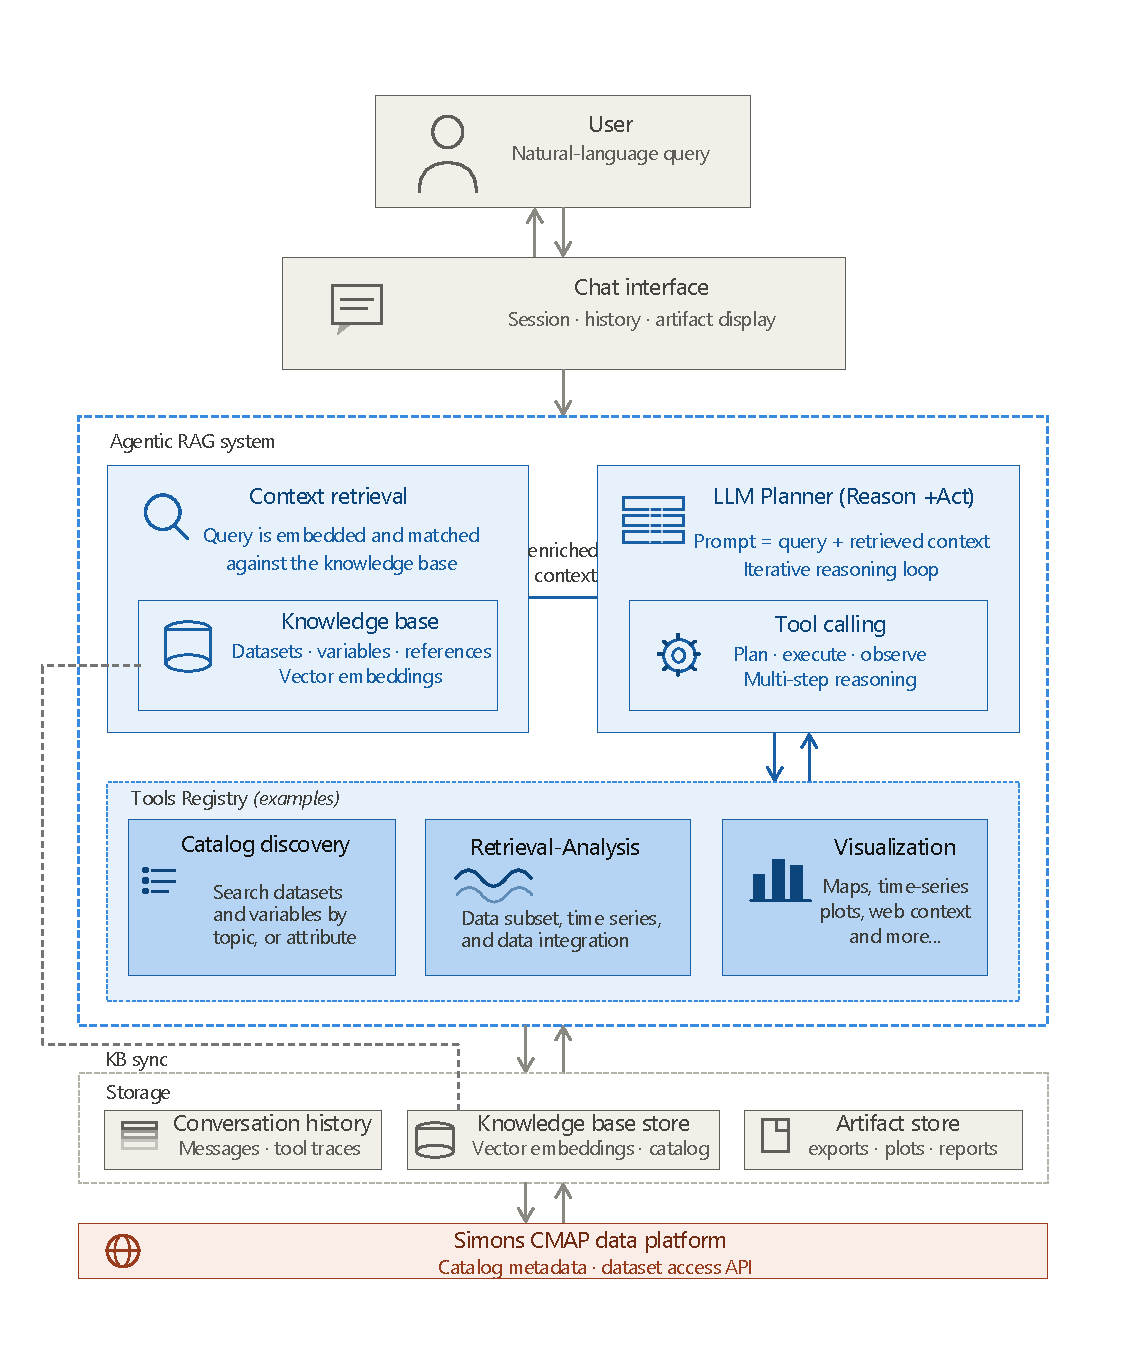
\includegraphics[width=\linewidth,height=0.6\textheight,keepaspectratio]{figures/architecture.pdf}
  \caption{Conceptual architecture of the conversational \cmapagent. User queries are processed through a Retrieval-Augmented Generation (RAG) pipeline that semantically searches a domain knowledge base---populated from the \cmap\ catalog---to enrich the prompt supplied to a foundation model. The model operates in an agentic loop, iteratively invoking specialized tools for dataset discovery, data retrieval, analysis, and visualization until a final response is synthesized. Conversation history, embeddings, and output artifacts are persisted across sessions, and the knowledge base is refreshed as the CMAP catalog evolves.}
  \label{fig:architecture}
\end{figure}

\paragraph{From intent to executable analysis.}
The system is designed to translate open-ended scientific intent (e.g., ``compare chlorophyll and SST seasonality in a region'') into a sequence of verifiable operations:
dataset/variable resolution, spatiotemporal subsetting, optional integration of multiple datasets, computation, and visualization.
Rather than asking users to learn internal catalog identifiers and calling conventions, the agent performs these steps while exposing intermediate decisions through tool traces and returned artifacts.

\paragraph{Grounding and verifiability.}
Two mechanisms are central.
First, retrieval over a curated knowledge base provides domain context (catalog entries, variable semantics, and usage guidance) to reduce hallucination and improve correct dataset selection.
Second, analyses are executed through explicit tools with constrained inputs and programmatic validation, so that computations and figures are produced by deterministic routines rather than free-form text.

\paragraph{Artifact-oriented outputs and reproducibility.}
Outputs are centered on scientific artifacts: subsets of data, figures, and (when appropriate) reusable code snippets that reproduce the same operations in the CMAP software ecosystem.
This design supports interactive exploration while enabling transition to scripted workflows for publication-quality analyses.

\paragraph{Separation of scientific semantics from implementation.}
While the system is realized as a concrete software stack, the scientific claims in this paper emphasize capability and behavior rather than the specifics of frameworks or deployment.
This separation is important for long-lived scientific infrastructure, where engineering choices may evolve while the user-facing semantics and provenance guarantees remain stable.
